\documentclass{article}
\usepackage{graphicx} % Required for inserting images

\usepackage{float}

\usepackage{dialogue}
\usepackage{tikz}
\usepackage{natbib}
\usepackage{setspace}
\usepackage{tabularx}

\usepackage{amsmath}
\usepackage{amsthm}
\usepackage{amssymb}

\newtheorem{theorem}{Theorem}
\newtheorem{proposition}[theorem]{Proposition}
\newtheorem{lemma}[theorem]{Lemma}
\newtheorem{definition}[theorem]{Definition}

\begin{document}
\title{The Task-Based View and Generative AI}
\author{John Horton\\MIT \& NBER}
\date{\today{}}

\newcommand{\machine}[1]{\langle #1 \rangle}
\newcommand{\human}[1]{( #1 )}
\newcommand{\cost}[1]{C\{ #1 \}}
\newcommand{\costdo}[1]{C_H\{ #1 \}}
\newcommand{\costmanage}[1]{C_M\{ #1 \}}

\newcommand{\topic}[1]{\paragraph{#1}}
%\newcommand{\topic}[1]{#1}

\maketitle

\begin{abstract}
\noindent The distinctive feature of generative AI is that it generates: code, writing, images, music, videos, and so on, and does so at essentially zero marginal creation cost.
These generations are made in response to some request or ``prompt.''
But these AI generations only become economic goods if judged suitable for some human need.
This depends on human judgment in the evaluation, the skill in crafting the prompt, and the technical capability of the generative model. 
When deciding to route a task to an  AI, the question is whether the prompt-evaluation loop inherent in using that AI will be more efficient than simply doing the task by hand. 
Tasks can be efficiently changed together, in the sense that each task feeds into the next without human intervention.
A task might be added to an automated chain even, if the human has an absolute advantage in that task in isolation.
\end{abstract}

\onehalfspacing

\section{Introduction}
\topic{Economic models on the effects of technology have to make simplifying assumptions about what that technology can and cannot do.}
The problem with generative AI---from an economic modeling standpoint---is that it is unclear what this kind of AI \emph{cannot} do even now, never mind over the next 5 or 10 years.
There is now talk about AGI that migth occur in our lifetimes.
As such, it seems prudent to move away from what AI cannot do and instead try to identify what is likely to be fundamentally human, no matter how much AI capabilities advance.

For example, \cite{autor2003skill}'s ``computation substitutes for routine cognitive tasks and complements non-routine cognitive tasks'' is a useful simplification of what computers do. 
Or technology automates some tasks previously done by humans but also spurs new tasks which only humans can do, at least for some time \citep{acemoglu2019}. 
Or AI is a prediction technology that lowers prediction costs, increasing the value added by labor that complements prediction \citep{agrawal2019}. 

Economists have framed advances in AI as advances in prediction technology \citep{agrawal2019}.
While forecasting and prediction are certain key firm tasks, relatively few workers have that as a task. 
By comparison, the outputs of generative AI---things like writing, research, or analysis (which could include prediction) are commonplace. 
As a case in point, on ONET, only 22 occupations are returned for the search term ``predicting.'' 
By comparison, the occupations returned for communicating, writing and analysis are 426, 332, and 408, respectively. 

\topic{There are contrasting ways consider the effect of technology on labor markets.}
One approach to understanding the impact of technology on labor markets has been to focus at the ``task'' level.
Goods are produced by the completion of tasks and those tasks can be assiged to the factor of production with the comparative advantage in that task.
This approach has been applied not just to technology, but also to trade and offshoring.
But specifically with respect to AIa nd automation, the task-based view is that labor, by being more flexible \citep{acemoglu2011skills}, has an absolutely advantage in ``new'' tasks, but that as time passes, they become susceptible to automation \citep{acemoglu2018}.

%\cite{acemoglu2022artificial}

A contrasting view if offered by \cite{bresnahan2020artificial}, who argues there has been no task level substition with the AI systems we actually see in production: ``The transition to ICT-based production has largely proceeded at the system level, not the task level.''
It has all been capital deepening.
To the extent there is important labor-capital substition, it will happen at the system level.
There is a long tradition in studies of ICT to take a ``systems'' view---that ICT requires a reconfiguration of production to reap the benefits (Cite Erik).

\topic{Generative AI certainly seems to be task-related and not just systems-related.}
The things it can do well: analyzing data, writing reports, drafting communications, doing research, coming up with plans, etc. certainly seem like the kinds of tasks common across large numbers of worker.
The product market success and adoption of ChatGPT is a testament to this: there are 100M users of OpenAI and presumably many are using it for their work.
Even the names of these technologies indicate their role of helping individuals: the names people use like ``co-pilot'' and ``assistant.'' 

\topic{The literature to date on AI specifically (as opposed to automation) has emphasized AI as a prediction technology \citep{agrawal2019}.} 
Although this is an area where machines can excel---and fit \cite{bresnahan2020artificial}'s examples perfectly---this seems, with hindsight, to be too narrow of a framing.
Generative AI models have shown the ability to create output similar to or better than even expert humans can produce over a broad class of knowledge-processing tasks.  
Consistent with this view, experimental evidence at knowledge worker tasks shows large productivity gains using ChatGPT for a collection of knowledge worker tasks \citep{noy2023experimental}.

They can do tasks that we would have thought impossible for computers to do even a short time ago.
Given these capabilities, it is widely anticipated that they \emph{will} have labor market effects, but what those effects are remains to be seen. 
We would like to have the generative AI version of \cite{autor2003skill}, but our problem is the same as if \cite{autor2003skill} tried to write their paper in 1960.
With the caveat that predicting the future is a mug's game, can we examine what these technologies do and try to sketch out the likely labor market implications now? 

\topic{The rise of generative AI has challenged the plausibility of older simplifications about the nature of AI.}
The fraction of tasks currently performed by workers in the US that might be done or augmented with LLMs is considerable \citep{eloundou2023gpts}.
The other problem is that these new technologies have not yet had their economic impact, so our historical data can tell us little about how technology is likely to affect the economy. 

\paragraph{Economic forces tend to create dependencies between tasks both within in a job and within a firm.}
From the time economists first recognized the division of labor as an important part of production, the interdependence between tasks has been noted.
The manufacture of pins proceeds linearly, with each step serving as an input to the next step in the productive process.
First the wire is washed and spooled, then pulled straight, then cut into lengths, then ground to a point, and so on.
A failure at any step jeoaparidizes the final product. 
This is at the heart of the \cite{kremer1993} o-ring model.

Tasks also have a recursive structure.
Every task can be divided into smaller sub-tasks.
For a human, we think of anyone as being able to ``do a task'' as also being able to do every constituent sub-task, in combination with the appropriate capital.
A machine might only be able to do some sub-set of those tasks. 
If tasks did not have a recursive structure, the division of labor would reach some atomic limit. 

Smith identified the limit to division of labor as not about hitting some atomic limit, but rather it was about the extent of the market. 
If you producing so much, you can employ one person or one machine doing the tiniest of tasks.
With a smaller market, less so.
But there is another cost, at least for labor: switching costs and communication cost.
When I hand off my output in some chain, if I need to explain what should happen next.

The logic of comparative advantage and communication costs tend to create serial dependencies between tasks within jobs, creating an o-ring-like production structure.
In the model, tasks within a job have serial dependencies. 
There are economic forces that push this characterization to be true. 
If a job lacked serial dependencies between tasks, we could likely reap more gains for specialization.
It costs us too much to hand off a task.
We only do it when we cannot do the task or the labor savings are so great it is worth it. 
The labor savings are great when management costs are low: the task is easy to describe, easy to evaluate, and has a high probability of success. 

For Coasian reasons, we also expect inter-dependencies between jobs within the firm.
%When we aggregate to level of the firm, things are not quite so linear.

A natural question is the delineation of these tasks---where does one begin and the other end? 
Tasks can be subdivided, with every step capable of being broken into smaller steps.\footnote{
    Writing a memo has the subtask ``write the first line of the memo'' then ``write the second line of the memo.''
    ``Write the first line of the memo'' and can be broken into ``first word'' and ``first letter'' and ``keystroke down, then keystroke up.''    
}
For our purposes, a helpful delineation is some sequence of tasks such that an AI could, in principle, do that whole sequence of constituent sub-tasks.
The capabilities of the AI model make the tasks. 
The start of the task is the first point where some human direction about what to do is required. 

\paragraph{Offering a system and task unified view}

\topic{The distinctive feature of generative AI is that it generates: writing, code, images, music, videos, and so on---but only in response to a human prompt.}
What the AI generates is not simply a random draw of things the AI could produce.
Rather, it produces something in response to some human request or prompt.

\topic{What AI generates is not inherently useful but rather depends on a human judgement.} 
The raw output must be evaluated and deemed suitable through judgment.
This assessment can then influence where the human asks the AI to modify the output in the required direction. 
This creates a human-AI hybrid loop of prompting and judging. 
And upstream of all of this is the necessary human insight into routing, or whether the task is one that an AI is likely to lead to a good outcome, with the prompting and evaluation the worker can provide. 

In addition to whatever others tasks for which a comparative advantage exists, no matter how capable these models become, two human tasks remain:
2) asking the AI to do that task, and 
3) evaluating the machine's efforts. 
Each of these steps is a human-provided task that can, in turn, be AI-augmented. 

\topic{This paper offers a way to unify a task- and systems-based view of AI and labor.}
Like in the task-based view, a productive process is a collection of tasks.
However, those tasks are assumed to be done in sequence, with interdependecies.
At each step, the task is given to the factor with the comparative advantage---though this can depend on what tasks are nearby.
But when a task is given to an AI, there is still human involvement in (1) communicating what is desired to the AI and (2) assess the output and potentially reformualting the preompt as needed.
The decision to route to an AI depends not only on the theoretical capabilities of the AI for a task, but how well the AI is likely to do, given the prompting and judgment of the human. 

If they choose to use an AI, the human asks the AI to perform the task with a prompt. 
The AI tries to perform the task, generating output.
The worker then evaluates the output to decide if it is suitable. 
If it is, the worker can continue to the next task 
If it is not, the human can try to modify the prompt and re-evaluate the new output until the need is satisfied. 

One might think that evaluation itself could be the domain of the AI, but if the model could have improved the chance the output would be evaluated positively, that process would have already been incorporated into the model. 
What is left is the residual evaluation that a human must uniquely supply: judgment.

There is no imposed structure on the kinds of tasks that humand and machines have advantages in.
If we want to assume a machine cannot do a task, we can assume it has a zero probability chance of completing the task; if we want to assume that a human cannot do a task, we can assume infinite cost.

\topic{The paper offers a computational model in that the allocation of tasks to factors happens within a sequence.}
Unlike the task-in-isolation view, it is possible to reap further benefits from automation even from tasks where humans have an advantage.
Namely, tasks can be ``chained'' together in automation to create entire ``systems.''
Note that with this chaining ``tasks'' can become increasingly large and abstract as models increase, generating something that looks like an entire ``system'' and not just a task.
As this occurs, what constitutes a ``task'' moves to higher and higher levels of abstraction: 
From ``find typos in this ad copy'' to ``create ad copy'' to ``create a marketing campaign, launch, execute and monitor performance'' to ``increase sales'' to ``run the business profitably'' to $\ldots$.  

The advantage of an automation system is that marginal costs can very, very low.
If having something produced is as simple as asking for it, costs can be very low indeed.
If some combination of tasks can be created so that there is no need for a human in the loop at any step, the whole process can be automated. 

\topic{There are numerous advantages to this computation approach to tasks.}
It matters what tasks are ``next'' to each other in some productive process, because tasks that have a high ability to be automated can be chained together.
As such, we can get ``automation dispersion'' where tasks are automated in some production settings but not others.

For example, consider the task ``answer questions about the text in a document'' and whether an AI can do this task depends on the payoff to doing it correctly. 
The firm might be fine letting a machine do low-level customer service support; we might be very hesitant to let it handle queries from major institutional investors, in part because what constitutes ``good enough'' might differ.
But also, the next task might be follow-questions about the state of the business that only the CFO can credibly answer.

This approach offers a point of view of what kinds of tasks are likely to be targets for automation---namely those that allow not just one-off task replacement but system-level replacement.
It also highlights that we are likely to see investment not only in direct model capabilities, but the ways in which they can be prompted and the results evaluated. 

The model gives another interpretation of the Acemoglu observation about so-so technologies: ```Examples of so-so technologies include automated customer service, which has displaced human service representatives but is generally deemed to be low quality and thus unlikely to have generated large productivity gains.''
While being able to replace human labor in some produce process can be cost saving, if the underlying technology is improving just incrementally and getting ``almost'' good enough, the benefit is likely to be small.
In contrast large jumps in model ability can have large effects, particularly if they facilitate chaining.

\topic{The model primitives map to things that can be measured.}
The time it takes to do a task; the task composition of a job; the capabilities of an AI in some area.
These are measuable things, and so the model is easy to take to data. 

\topic{The prompting/evaluating distinction gives us a new way to think about human complementarities to AI.}
Prompting is really the human skill of getting what you want out of some AI system.
There is no inherent reason to think that this will itself be a low-skill job---just a different skill job.
Most of management is deciding what you want done, asking right people to do it, in a way that leads to an effective outcome, and then monitoring the process to see if it acheiving the desired goals.
No one thinks of this as a ``low skill'' propostiion.

\topic{The literature on the cost of evaluation of goods---search goods, inspection goods, experience goods, credence goods---gives us an economic think about what tasks are are likely to be automated.}

\topic{It gives us a new way to think about changing who is eligible to fulfill some role in the productive process.}
To the extent there is some different in the requirements to do some task, ask for some task to be done, and evaluating the output of that ask, there is a possibility to use different kinds of workers in a productive task.

The approach gives a way to think about an occupation ``disappearing.''
In the model, an occupation only disappears when all of its task are subsumed in an automation chain.
Take an job that truly disappeared: elevator operator. 
The tasks were 1) ``Announce the direction of the elevator,'' 2) ``ask people what floors they are going to'' 3) ``bring the elevator to the appropriate floors'', 4) ``open the doors'' as well as some other non-sequential tasks like inspect for defects or machine failures.  
This got turned into an automation chain where the customer was given the ``prompting'' task of selecting a floor; the evaluation task is just seeing that the elevator was the appropriate floor---an inspection good with a low $c_e$.
If it was hard to know if you had gotten the right floor, we might expect that task to still be done by humans.

Although there are advantages to thinking in terms of tasks, most labor market participants thing in terms of ``occupations.'' 
Our training and human capital acquistion is structured as occupations.
People want to know which whole occupations will disappear, and what occupations have good prospects. 

\paragraph{A fully human task that remains has no economically viable sub-tasks to send to an AI.}

Suppose there is some sub-task of a human task that takes $c_h'$.
That the task is not broken down further implies that $c_h' < c_m / q$ for that task. 
It means there is no sub-task for which 


\paragraph{Jobs with few tasks are more prone to full automation}
All else equal, a job with a single task is more prone to automation compared to one with multiple distinct tasks.

\paragraph{Jobs where the next task is unpredictable are more resistant to full automation}
The benefits to combining multiple tasks into an automation ``chain''
But if task 1 and task 2 rarely occur together, chaining them together is not likely to work well if that requires some set up.

\paragraph{Serial correlation in AI features of tasks types facilitates chaining}

\paragraph{Net effects on labor}

As an information good, competition seems likely to push marginal costs of using these tools to zero.
There might be tasks that have a zero sumness where people will pay a premium for the very best models.

One might argue there will be increases in employment in developing AI tools, but consider that OpenAI has less than a thousand employees.\footnote{ 
  https://www.linkedin.com/company/openai/
}
The most likely effects will be due to productivity effects.
The new products that can be created when costs are lower.

\paragraph{Generative AI is an information goods factory, but it has human workers.}
Generative AI is that it works with us to produce information goods. 
And the economic-so-what is that the machines can do their part of the productive process at zero marginal cost---or at least at a cost that will likely trend to zero.

Digitization already pushed the marginal reproduction costs and distribution costs for information goods to zero---but the costs of initially producing those goods remained high: I could costlessly share an ebook with you, but writing a book was still a long, hard slog.

A prediction is an information good. 
But it is also an experience good that might reveal its quality over a long time frame, depending on the nature of the prediction. 
Once you know a prediction is good; it is probably useless other than as a data point that you should value the predictions of the machine more.
If it is a prediction about what might happen, but that could be changed given the firm's actions, it could be a credence good.
This is precisely the kind of task that the relative benefit of using an AI might be quite low if the ability to judge is low. 

\paragraph{Using an AI for some task has qualitative similarities to delegating a task to another human or team.}
The decision to use an AI bears similarities to the decision to delegate some task to a subordinate.
And conditional upon delegation, the skill of using AI bears similarities to the management of people and teams. 
Deciding whether the output is sufficient requires judgment, whether the output is human-produced or otherwise. 

\paragraph{Goods differ in their cost of human evaluation, which changes the cost of using AI for production.}
The extent of generative AI usage depends on the costs of judging the model's output.
This cost could vary considerably based on the nature of the good.
An analogy is drawn to the process by which consumers evaluate goods. 
Search goods are trivially easy to evaluate (and hence ideal candidates for AI creation), whereas inspection goods and credence goods might have prohibitively expensive evaluation costs. 
These differences will affect the adoption of AI by task.

\paragraph{Entrepreneurial innovation will focusing reducing AI management tasks as well as increasing model abilities}
We will see investment to improve the capabilities of models but also try to reduce the costs of prompting and to reduce the cost of the evaluation. 
The skills that AI complements are themselves potential targets for AI assistance. 
We will likely see AIs that help write prompts or make it easier for humans to express themselves.  
We will see AIs and related technologies that help evaluate output. 

\paragraph{AI will create new labor-labor substitution possibilities for ``Rick Rubin'' reasons.}
In light of the change in what is delegated, I discuss how labor-labor substitution might change who performs a task. 
In particular, job redesign will take advantage of the fact that skills in judging output are separate from the skill of creating some output.
There are food critics who cannot cook; record producers who cannot play instruments; technologists who cannot program, and so on.
As AI makes it so that humans no longer have to do every task in a job, AI might open up jobs to people who are otherwise blocked by a skill they lack.

There are likely to be numerous tasks when prompting and judgment can lead to good outcomes even when the human offering those judgments cannot do it themselves.
One reason is that the pool of people who can offer judgment is larger than the pool that can do the task. 
This might be particularly true for tasks that require a great deal of skill.
As a recent illustrative example,  the famed record product Rick Rubin described his value in a recent interview with Anderson Cooper:
\begin{dialogue}
\speak{Rick Rubin} I’ve no technical ability. And I know nothing about music
\speak{Anderson Cooper} Well, you must know something.
\speak{Rick Rubin} I know what I like and what I don’t like. I’m decisive about what I like and what I don’t like.
\speak{Anderson Cooper} So what are you being paid for?
\speak{Rick Rubin} The confidence that I have in my taste, and my ability to express what I feel, has proven helpful for artists.
\end{dialogue}

However, that task has to be marginal (assuming other blocking tasks are not also automated). 
For example, identifying a bone fracture in an X-ray does not mean a person is ready to be a radiologist.
I.e., if there was only one task that precluded them from doing some occupation, then AI might allow them to do that occupation.
Allowing more people to do more tasks could have an indirect productivity effect. 
Ironically, the harder the task to perform, the more potential for AI to unlock this substitution potential, as the pool of potential prompters and judges is much larger than the pool of doers.

\topic{Generative AI might allow for a kind of pseudo-human capital acquistiion.}
Substitution to another human might require a hand-off if all the rest of the tasks still need to be done by the ``original'' human. 
But AI augmentation might allow for a task re-design. 
Consider that for some occupations, there are necessary tasks such that $c_h$ is essentially infinite, or so high that it would be uneconomic for that person to pursue that job because their effective efficiency wage would be lower than their next best alternative.  
Take, for example, a master carpenter versus a handyman.
There are many tasks in common between the two: driving to the job site, carrying tools, buying supplies, swinging a hammer, etc.
But what is distinguishing is that there are tasks required of the master carpenter that the handyman is incapable of performing. 
This drives down their wage below the handyman wage, and so they are handymen.
If generative AI is inequality-reducing, I think this will be the mechanism: taking people that currently lack certain skills and letting them ``jump'' up. 

This framing gives an interesting characterization of the human capital acquisition process  generally: learn skills that will lower your performance costs across tasks \emph{if} you can make the job requiring those tasks better than your best job option.
The skills you acquire need to make that job marginal. 
For example, the task ``read an MRI scan to detect a bone fracture'' is highly remunerative but only if learned in with all the other tasks in the ``Radiologist'' task sequence.
Licensing aside---this skill alone is essentially worthless.  
With AI augmentation, the marginal blocking skill might no longer be blocking. 

\paragraph{Generative AI substitutes ``maker labor'' and complements ``manager labor'' in the short-run.}
In the model, there are just two broad ``kinds'' of labor: 
Labor that does tasks, and labor that manages an AI doing that task. 
While we might think there is some correlation between the cost of the machine and the human doing the task, this seems like an imprudent assumption.

We should not presume that tasks that are hard for humans are easy for computers or vice versa. 
We do hard, time-consuming tasks because the output is valued. 
Playing excellent chess \emph{seemed} like the kind of thing computers can do well. 
Generating photorealistic art, playing diplomacy, and generating new programs on the fly did not seem like tasks where computers would show capabilities.

All else equal, more capable management increases the number of tasks an AI performs, holding AI capabilities fixed. 

Being adjacent to a highly automatable task will tend to ``pull'' that task into an automated chain.


\section{A model of production}
To start, imagine a job that consists of just a single task: task 1.
A human can do the task at a cost of $c_h$.
An AI that can \emph{try} do the task instantly at zero cost and if ``prompted'' by a human.
However, it it only succeeds with probability $q$, given the optimal effort by the human at ``prompting.''
This $q$ captures the model's capability but also reflects the capability of the human at prompting and judging.
Each prompt costs the human $c_p$, and each evaluation of an AI output costs the human $c_e$.
Let $c_p + c_e = c_m$, with $m$ for ``management.''

If the machine fails at a task, it is kicked back for the human to try again with another prompt, at another cost of $c_p$ and then $c_e$.
Success and failures are independent, and so it always makes sense to keep trying with the AI, conditional upon it making sense to try once.


To indicate a task being done by a human, we will use the notation $\human{\cdot}$.
For a task don by a machine, we use the notation $\machine{\cdot}$.
As a memory aid, note the curved parenthesis captures of $\human{\cdot{}}$ the greater ``flexibility'' of humans. 
Figure~\ref{fig:flow} illustrates the situation.

\begin{figure}
\caption{A job with a task decomposed into sub-tasks} \label{fig:flow}
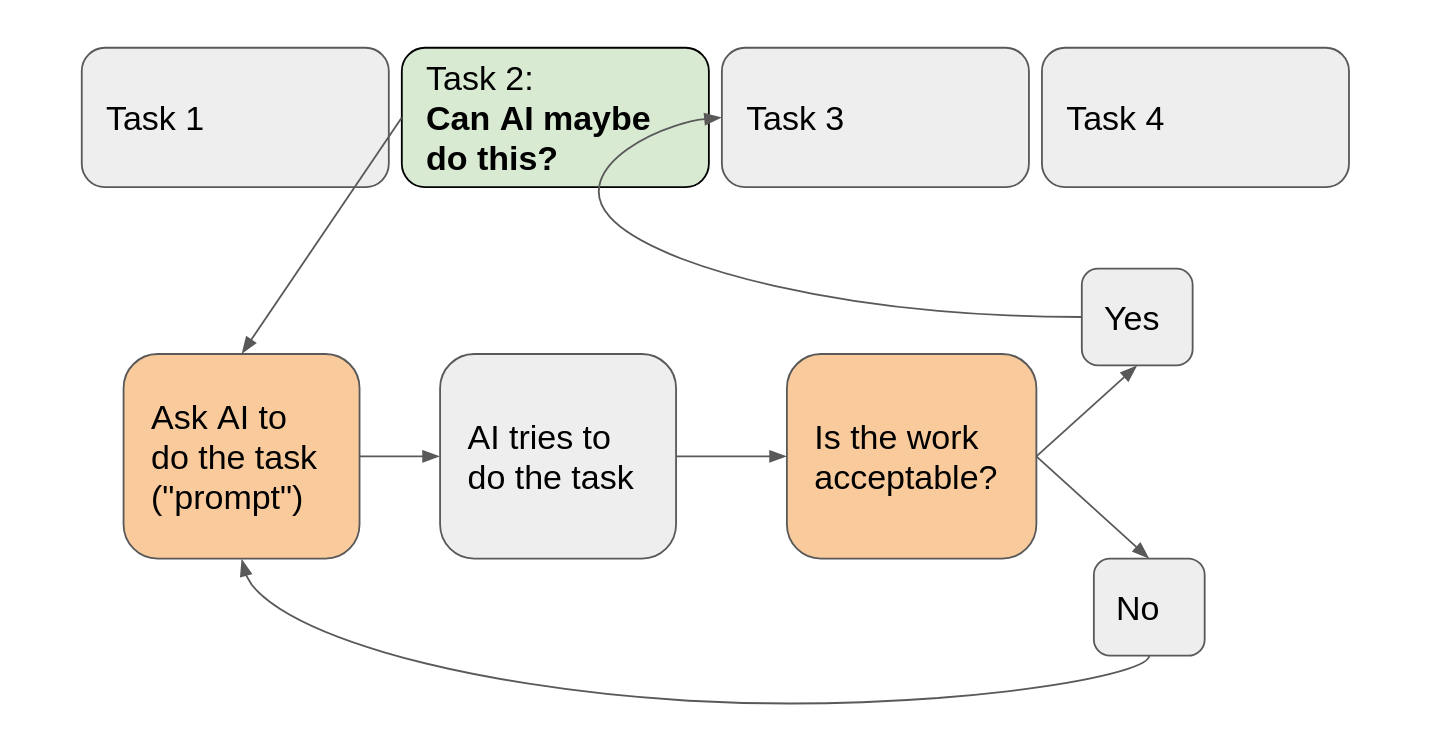
\includegraphics[width = \textwidth]{flow.png}
\end{figure}

Lemma~\ref{lemma:when} gives the criterion for automation when considering a task in isolation: is $c_h > c_m / q$.

\begin{lemma} \label{lemma:when}
 For a given task, it is cheaper to automate if $\cost{\machine{1}} < \cost{\human{1}}$, which happens when $c_m / q < c_h$.
\end{lemma}
\begin{proof}
  The expected cost of using the AI for a task is $c_m/q$.
  Recall
  \begin{align}
    \sum_{k=1}^\infty k q^k (1-q)^{k-1} = 1/q,
  \end{align}
and so the task will be automated if $q > \frac{c_m}{c_h}.$
\end{proof}

This decision criterion has some intuitive properties.
The higher the human performance costs, the more likely a worker is to try an AI, even a fairly incapable one (i.e., low $q$).
The lower the prompting and evaluation costs, the more likely an AI will be used.
If we think of novice workers as having higher own-performance costs, or high $c_h$ values, they might be more likely to use an AI.

Note that we are ignoring capital costs---all that are present are labor costs.
Note that with a high capable AI $(q = 1)$ that is very easy to use ($c_m \approx 0$), costs can be very low.

In isolation, raising $q$ has two effects on labor.
It displaces direct labor, as it is more likely that $c_m/q < c_h$, but increases the demand for management-labor of the extensive margin, as more tasks flip from being done by a human to being done by a machine.

This constant $q$ even for a single task is a simplification, as we might expect the ``first'' $q$ to be low for a given prompt, but then increase with each subsequent prompt that is a refinement.
However, it will still have a finite expectation.

It seems likely, empirically, that prompting costs are sub-linear with respect to $c_h$ for many tasks.
The prompt ``write me a haiku about economics'' is about the same effort as ``write me an epic poem about economics'' but the $c_h$ differs radically. 
To the extent $c_h$ and $c_e$ vary less than $c_h$, we should expect a size bias, with more attempts to use for larger tasks in the $c_h$ sense.  

\subsection{A job with two tasks}
Now imagine two tasks, 1 and 2, with AI success probabilities $q_1$ and $q_2$, respectively.
The 4 human/machine possibilities are: both tasks are done by human, $\cost{\human{1}\human{2}} = 2 c_h$;
both are done by machine, $\cost{\machine{1}\machine{2}} = c_m (1/q_1 + 1/q_2)$;
task 1 by a machine and task 2 by hand, $\cost{\machine{1}\human{2}} = c_m/q_1 + c_h$; and task 1 by hand and task 2 by machine $\cost{\human{1}\machine{2}} = c_h + c_m/q_2$.

We now introduce another possibility: the ``chaining'' of AI tasks.
Doing this creates a new task with a success probability equal to the product of the success probabilities of the constituent tasks.
It is similar to \cite{kremer1993}'s model of production.
The chained-together task still has human prompting and evaluation at the start and end, inheriting the $c_p$ of the first task and the $c_e$ of the last task.
Notation-wise, a ``$|$'' indicates chained-together tasks, e.g.,  $\machine{1|2}$ indicates a machine does tasks 1 and 2 in sequence.
This creates a fifth possibility in the two-task scenario, $\cost{\machine{1|2}} = c_m/(q_1q_2)$.

For a given task $k$, we can think of $q_k$ as the probability of success when it gets a perfect input.
When a human did the preceeding task or a human managed the AI process, $\machine{k-1}$ or $\human{k-1}$, the task is done perfectly.
In contrast, when the asks are chained, $\machine{k-1|k}$, there is no quality assurance between tasks, and so the probability that the $k$ task gets a perfect hand-off is only $q_{k-1}$.

Figure~\ref{fig:diagram} illustrates the possibilities with the unit square, with $q_1$ on the x-axis and $q_2$ on the y-axis.
It is a contour plot showing costs of production.
For purposes of example, both tasks have same human cost and management costs, $c_h = 3/2$ and $c_m = 1/2$. 
The unit square is divided into five regions, corresponding to the five possibilities for a two-task job.

\begin{figure}
  \caption{Production costs with a two task job} \label{fig:diagram}
  \centering
    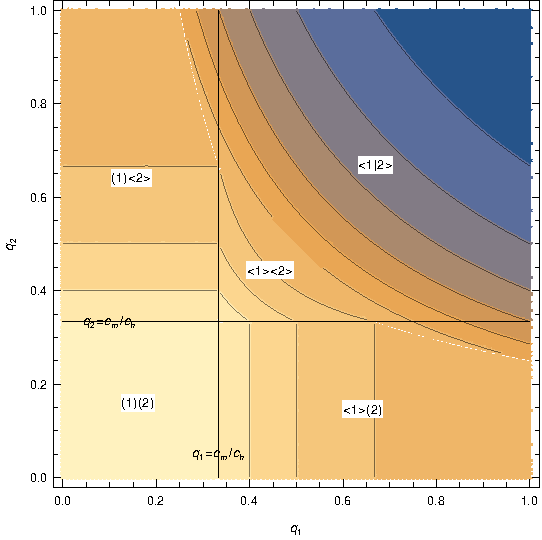
\includegraphics[width = 0.7 \linewidth]{images/diagram.pdf}
\end{figure}

In the human-only $\human{1}\human{2}$ region, there is no gradient with either $q_1$ or $q_2$, as the AI capabilities are irrelevant.
It is flat plateau of costs $2c_h$.
In the partial automation regions, there is a gradient in cost with respect to the automated task: $\frac{d \cost{\human{1}\machine{2}}}{dq_2} < 0$ and $\frac{d \cost{\machine{1}\human{2}}}{dq_1} < 0$, but zero cross partials.
This is also true in the automated-but-not-chained region of $\machine{1}\machine{2}$.

In automation chains, investments in either task help, but interstingly, they have cross-partials in terms of cost reduction that make them substitutes.
We can so that with $\frac{d}{d q_1 q_2} \cost{\machine{1|2}} = \frac{1}{q_1^2q_2^2}$.
In other words, an investment in $q_1$ is, all else equal, worth more when $q_2$ is low.
This feature would tend to create incentives for ``balanced'' investment in tasks, trying to improve the weakest link in the chain.

Interstingly, with $\machine{1|2}$, there are regions where humans have a comparative advantage in a task ($q < c_m/c_h$), but it is still fully-automated because of the advantages of chaining together tasks.
The $\human{1}\machine{2}$ to $\machine{1|2}$ boundary and the $\machine{1}\human{2}$ boundary are intersting:
the curves are define by $c_h + c_m/q_2 = c_m/(q_1q_2)$ and $c_h + c_m/q_q = c_m/(q_1q_2)$, respectively.
At the boundaries, humans actually have a comparative advantage in the task compared to a machine \emph{alone}, but the possibility of chaining ``pulls'' this task into full automation. 

Lemma~\ref{lemma:ce} shows that the automation decision cannot be made in isolation and that it depends on the adjacent tasks.

\begin{lemma} \label{lemma:ce}
A task might be automated even if humans have a comparative advantage over machines in doing that task:
$C\{\human{1}\machine{2}\} < C\{\machine{1}\machine{2}\}$ does not imply $C\{\human{1}\machine{2}\} < C\{\machine{1|2}\}$.
\end{lemma}
\begin{proof}
We can see this with a counterexample.
The machine success probabilities are $q_1 = 3/5$ and $q_2 = 4/5$.
Management costs are the same for both tasks, $c_m = 1$.
Human performance costs for the first task is $c_h = 3/2$.
Let the human performance cost for the second task be $\infty$, so it must be automated. 
Note that for the first task, it is cheaper to have the human do it: 
$c_h < c_m / q_1$, as the human cost is just $3/2 = 9/6$ but the AI cost is $5/3 = 10/6$.
However, we fully automate the costs are 
$c_m / (q_1 q_2) = 25/12$. 
If we do the first by hand and automate the second, we have total costs of $c_h + c_m / q_2 = 11/4$, or $33/12$.
Thus, even though humans have a comparative advantage in a task, we might chain it with another task and manage the combined task.
\end{proof}

\subsection{When to chain to tasks}
The decision to chain two automated tasks is simple: chain if $q_1 + q_2 > 1$.
This is given in Lemma~\ref{lemma:chain}.

\begin{lemma} \label{lemma:chain}
If $q_1 + q_2 > 1$ and $\cost{\machine{1}} < \cost{\machine{1}}$ and $\cost{\machine{2}} < \cost{\machine{2}}$, then $\cost{\machine{1|2}} < \cost{\machine{1}\machine{2}}$.  
\end{lemma}
\begin{proof}
If we chain the tasks, costs are $\frac{c_m}{q_1q_2}$, whereas if we split them up, we have $\frac{c_m}{q_1} + \frac{c_m}{q_2}$.
We chunk to tasks if 
\begin{align}
\frac{1}{q_1 q_2} <\frac{1}{q_1} + \frac{1}{q_2}
\end{align}
which is true when $q_2 + q_1 > 1$, otherwise they should be split. 
\end{proof}

A related implication of Lemma~\ref{lemma:chain} is that the success probabilities of each task must sum to greater than 1 as a necessary--but not sufficient---condition for a chain.

\begin{lemma} \label{lemma:sum1}
A cost-minimizing sequence, $T^*$, cannot have a chained machine sequence with sum of $q$ values less than 1.
\end{lemma}
\begin{proof}
Suppose we have a chain in $T'$ with $Q = q_1 q_2\ldots q_k$ and that $\sum_k q_k < 1$ and that it is cost-minimiziing i.e., $T' = T^*$.
Take the smallest $q$ internal to the chain and call it $q_\epsilon$.
We can treat the situation as a three-chain problem, $q_l$, $q_\epsilon$ and $q_r$, with $l$ and $r$ for left and right.
The fully automated chain has greater costs that the ``separated'' chain $\cost{\machine{l|\epsilon|r}} > \cost{\machine{l}\machine{\epsilon}\machine{r}}$ if
\begin{align}
  \frac{1}{q_lq_{\epsilon}q_r} > \frac{1}{q_l} + \frac{1}{q_\epsilon} + \frac{1}{q_r}  \nonumber \\
   \frac{1}{q_lq_{\epsilon}q_r} > \frac{q_r q_\epsilon}{q_l} + \frac{q_rq_l}{q_\epsilon} + \frac{q_lq_\epsilon}{q_r} \nonumber \\
   1 > q_r q_\epsilon + q_rq_l + q_lq_\epsilon \nonumber,
\end{align}
and because $q_l + q_\epsilon + q_r < 1$, and all $q$ values are less than or equal to 1, $1 > q_r q_\epsilon + q_rq_l + q_lq_\epsilon$.
Therore, $T'$ is not the cost-minimizing sequence.
\end{proof}

Lemma~\ref{lemma:sum1} will prove useful later for computing cost-minimizing allocations, as it allows us to further prune the tree.  

\begin{lemma} \label{lemma:pair_better}
If a task can be combined with either a more or less reliable chain, if it should be combined, it should be combined with the more reliable chain.
 If $\cost{\machine{1}} > \cost{\machine{3}}$, then $\cost{\machine{1}\machine{2|3}} < \cost{\machine{1|2}\machine{3}}$.
 \end{lemma}
\begin{proof}
Suppose you have $q_L$, $q$, and $q_H$, in sequence, with $q_H > q_L$.
Assuming you will chunk left or right, which chunk to you choose?
\begin{align}
 \frac{1}{q_L} + \frac{1}{q q_H} < \frac{1}{q_L q} + \frac{1}{q_H} \\
  q q_H + q_L < q_H + q q_L \\
  q (q_H  - q_L) < q_H - q_L.
\end{align}
\end{proof}

Humans can ``hand-over'' tasks to an AI---but can the AI hand over tasks to the human?
In the model, when a chain goes from $\human{0}\machine{1|2}\human{3}$, we can think of the human as handing off tasks 1 and 2 to the machine, but we can also think of the machine as handing off task 3 to a human.

\subsection{Multiple tasks}
Now we will consider a job that is a sequence of tasks to be performed $1, 2, \ldots n$.
Here, we will focus on the computational aspects of the problem.

Let $C_h$ be a vector of costs to a human for performing each task.
%% Consider an $n = 5$ job. 
%% If $\machine{1|2}\human{3}\human{4}\machine{5}$, it would indicate tasks 1 and 2 done in a chain by a machine.  
%% The per-pass success probability of $\machine{1|2}$ is $q_1q_2$. 
%% Tasks 3 and 4 would be done by humans, while task 5 would be done by an AI. 
%% Total costs for the good would be $\frac{c_m}{q_1 q_2} + c_{h(3)} + c_{h(4)} + \frac{c_m}{q_5}$.
Note that with an $n$ task jobs, there are $2^{n-1}$ possible task partitions.
And each singleton can be done by a human or a machine; each sequence is done only by a machine.

The cost minimization problem is equilvalent to finding the shortest path in a tree.
To grow the tree, start with the first task.
It can be automated or done by a human.
It then has up to two children---the next task is either machine or human, and if machine, it could also be part of a chain.
Figure\ref{fig:tree} illustrates the tree. 

The tree grows to, worse-cast, $2^n$ children where $n$ is the number of tasks.
It would be less than this because human-done nodes only have one child: either machine or human.
Growing the tree has an exponential computation complexity---it is unclear if there is a polynomial time algorithm.
It might also be possible to prune certain leafs using the logic of Lemma~\ref{lemma:sum1}.

\begin{figure}
\caption{The possible production scenarios with an $n=2$ task job}
\label{fig:tree}
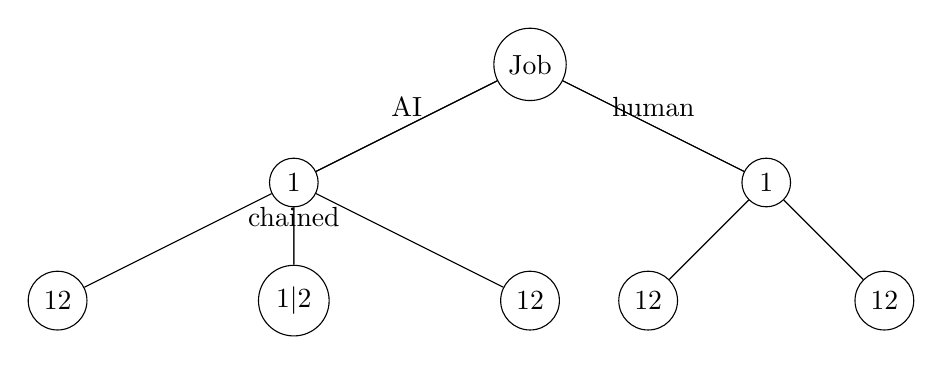
\begin{tikzpicture}[
  level/.style={sibling distance=60mm/#1}
]
\node[circle, draw] (S) at (0,0) {Job}
  child {node[circle, draw] (A) {$\machine{1}$}
    child {node[circle, draw] (AA) {$\machine{1}\machine{2}$}}
    child {node[circle, draw] (AAC) {$\machine{1|2}$}} 
    child {node[circle, draw] (AH) {$\machine{1}\human{2}$}} 
  }
  child {node[circle, draw] (H) {$\human{1}$}
    child {node[circle, draw] (HA) {$\human{1}\machine{2}$}}
    child {node[circle, draw] (HH) {$\human{1}\human{2}$}}
  };
\path (S) edge node[midway, above] {AI} (A);
\path (S) edge node[midway, above] {human} (H);
\path (A) edge node[midway, above] {chained} (AAC);
\end{tikzpicture}
\end{figure}

\section{Product market sketch}
Suppose there are $N_K$ tasks an economy which can be configured into $N_S$ slots.
This economy has ${N_K \choose N_S}$ possible products.
Let $d_i(p)$ be the quantity demanded for good $i$ when the price for that good is $p$.
This has an associated wage bill of $d_i(p) T^*_i$.
Of those products actually pursued in equilibrium, the price equals the cost: $p_i = \cost{T^*_i}$. 
Goods that are not produced at all are those where $d^{-1}_i(1) < \cost{T^*}$.
We could imagine many products are not produced because no one wants them at all, but others are just not price competetive.

Products that are produced have constant returns to scale.
All workers can provide the management input at $c_m$, which is the same for all tasks.
Before automation, the cost of each job is simply the sum of the costs of each task.

Workers optimally choose what subsets of the $K$ skills to acquire.
Although they could acquire $2^K$ possible bundles of skills, they only acquire those correspond to products actually produced in equilibrium.  

The cost to produce the item is $c_i = \cost{T^*_i}$, which is also the wage bill, as the only cost in the model is labor.
An increase in productivity raises output, which lowers prices.
With lower prices, more quantity is produced. 
An improvement in AI pushes out the frontier of products that are produced, as some are now cost effective.
Consumption is biased towards goods where AI can substitute for labor---particularly those with lots of chaining possibilities.

To make this more concrete, assume a single task, $k \in K$, can be automated, with say $q$ increasing dramatically.
Let $I$ be the set of all jobs that required skil $k$.
That set of jobs $I$ now demand less labor, for the same amount of output.
However, there is a productivity benefit from increased output that increases labor market demand.
Which one ``wins'' depends on the elasticity of the demand curve at the equilibrium price.
Demand for other skills that appear in $I$ jobs also decreases due to automation chains.

Consider that with $k$ automated, there are other workers who could now potentially compete for jobs in $I$.
Let $I_H$ bet the set of jobs where $k$ was the only skill workers there were ``missing.''
These are Rick Rubins.
This is a positive labor supply shock to the $I$-tasks market.
But it is a different supply shock in the $I_H$ markets---those that were paying higher wages will likely see an increase and wages wall, those that were paying lower wages will likely see wages rise---it depends on where they were prior to the collapse.
This is just Baumol's cost disease due to rising productivity in the $I$ sector.
By raising $c_h$ in $I_H$ sector, that increases the incentives to invest in automation.

The automation of $k$ also has impacts on the space of products produced in equilibrium.
Tasks with high $k$ costs might now become feasible, with tends to increase demand for labor with skills that complement $k$---which are precisely the skills those workers specializing in $k$ also had. 


\begin{proposition}
Lowering costs of any kind does not reduce the number of viable products.
\end{proposition}

\begin{definition}
An improvement in AI is when there exists a $j$ such that $Q'_i > Q_i$ and for all other indices $j$, $Q'_j \ge Q_j$
\end{definition}

\begin{proposition}
An improvement in AI capabilities does not increase costs: ${\cost{T^*_{Q'}} \le \cost{T^*_{Q}}}$.
\end{proposition}
% NB: There is some assumption to be made about distribution of tasks and costs such that costs decrease


\begin{lemma}
  Total costs stay the same or decline in $c_h$ and $c_m$.
  Both are likely sub-linear because of substitution possibilities.
\end{lemma}

\begin{lemma}
  Management labor and doer labor are gross substitutes.
\end{lemma}

\begin{lemma}
  Lowering the cost of AI has mixed effects on the demand for management labor; unambigous negative effects on doer labor.
\end{lemma}
\begin{proof}
  A decrease in $q$ raises the number of tasks automated, which increases demand for management labor.
  But it also reduces management costs, $\frac{d}{d q} \frac{c_m}{q_m} = -\frac{c_m}{q_m^2}$.
\end{proof}

\begin{proof}
  If $c_m$ decreases, demand for do-er labor decreases, lowering $c_h$ in equilibrium.
\end{proof}

\begin{lemma}
Increases in capabilities of AI (lower $q$) (a) deceases costs of existing goods, (b) expand the goods that are economical to produce in equilibrium, (c) give workers more income to purchase goods.  
\end{lemma}

\section{Model simulations}

I ran a simulation of many ``jobs'' with chained tasks and found
the lowest cost combination under different assumptions about human
and machine labor.
Human costs were fixed $c_h = 1$. 
I draw the $q$ from a unform distribution between $U[q_{min}, 1]$,
varying $q_{min}$.
The number of tasks in the chain was $n$.
$c_m$ was changed in each simulation, ranging from $0.1$ to $2$, in
$0.1$ increments.
The simulation parameters are: 

\begin{verbatim}
    num_sim = 100
    nrange = range(2, 11)
    cmin_range = np.arange(0.1, 2, 0.1)
    qmin_range = np.arange(0.1, 1, 0.1)
    cm_range = np.arange(0.1, 2, 0.1)
    n_range = range(2, 11)
\end{verbatim}

You can see how in the simulation, average task costs fall with longer chains.
This is presumably because longer chains can be full automated.

When AI management costs are higher, more tasks are done by humans.
When AI quality is higher, more tasks are done by machines.


\begin{table}[!htbp] \centering 
  \caption{Effect of costs and quality on outputs} 
  \label{tab:outcomes} 
\footnotesize 
\begin{tabular}{@{\extracolsep{-6pt}}lccc} 
\\[-1.8ex]\hline 
\hline \\[-1.8ex] 
 & \multicolumn{3}{c}{\textit{Dependent variable:}} \\ 
\cline{2-4} 
\\[-1.8ex] & Avg. cost/task & \multicolumn{2}{c}{Frac tasks by human} \\ 
\\[-1.8ex] & (1) & (2) & (3)\\ 
\hline \\[-1.8ex] 
 Num. tasks & $-$0.016$^{***}$ &  &  \\ 
  & (0.001) &  &  \\ 
  Management Cost &  & 0.362$^{***}$ &  \\ 
  &  & (0.002) &  \\ 
  AI model floor (qmin) &  &  & $-$0.633$^{***}$ \\ 
  &  &  & (0.006) \\ 
  Constant & 0.814$^{***}$ & $-$0.084$^{***}$ & 0.594$^{***}$ \\ 
  & (0.006) & (0.003) & (0.003) \\ 
 \hline \\[-1.8ex] 
Observations & 29,241 & 29,241 & 29,241 \\ 
R$^{2}$ & 0.009 & 0.457 & 0.310 \\ 
\hline 
\hline \\[-1.8ex] 
\end{tabular}
\\
\begin{minipage}{ \textwidth}
{\footnotesize \emph{Notes}: Some notes.}
\end{minipage}
\end{table}


Figure~\ref{fig:avg_cost_by_management_cost} shows that average prices increase in management costs (unsurprisingly) but that that the relationship appears to be either concave or convex depending on the baseline level of model quality.

\begin{figure}
\caption{Average costs versus management costs, by model quality} \label{fig:avg_cost_by_management_cost}
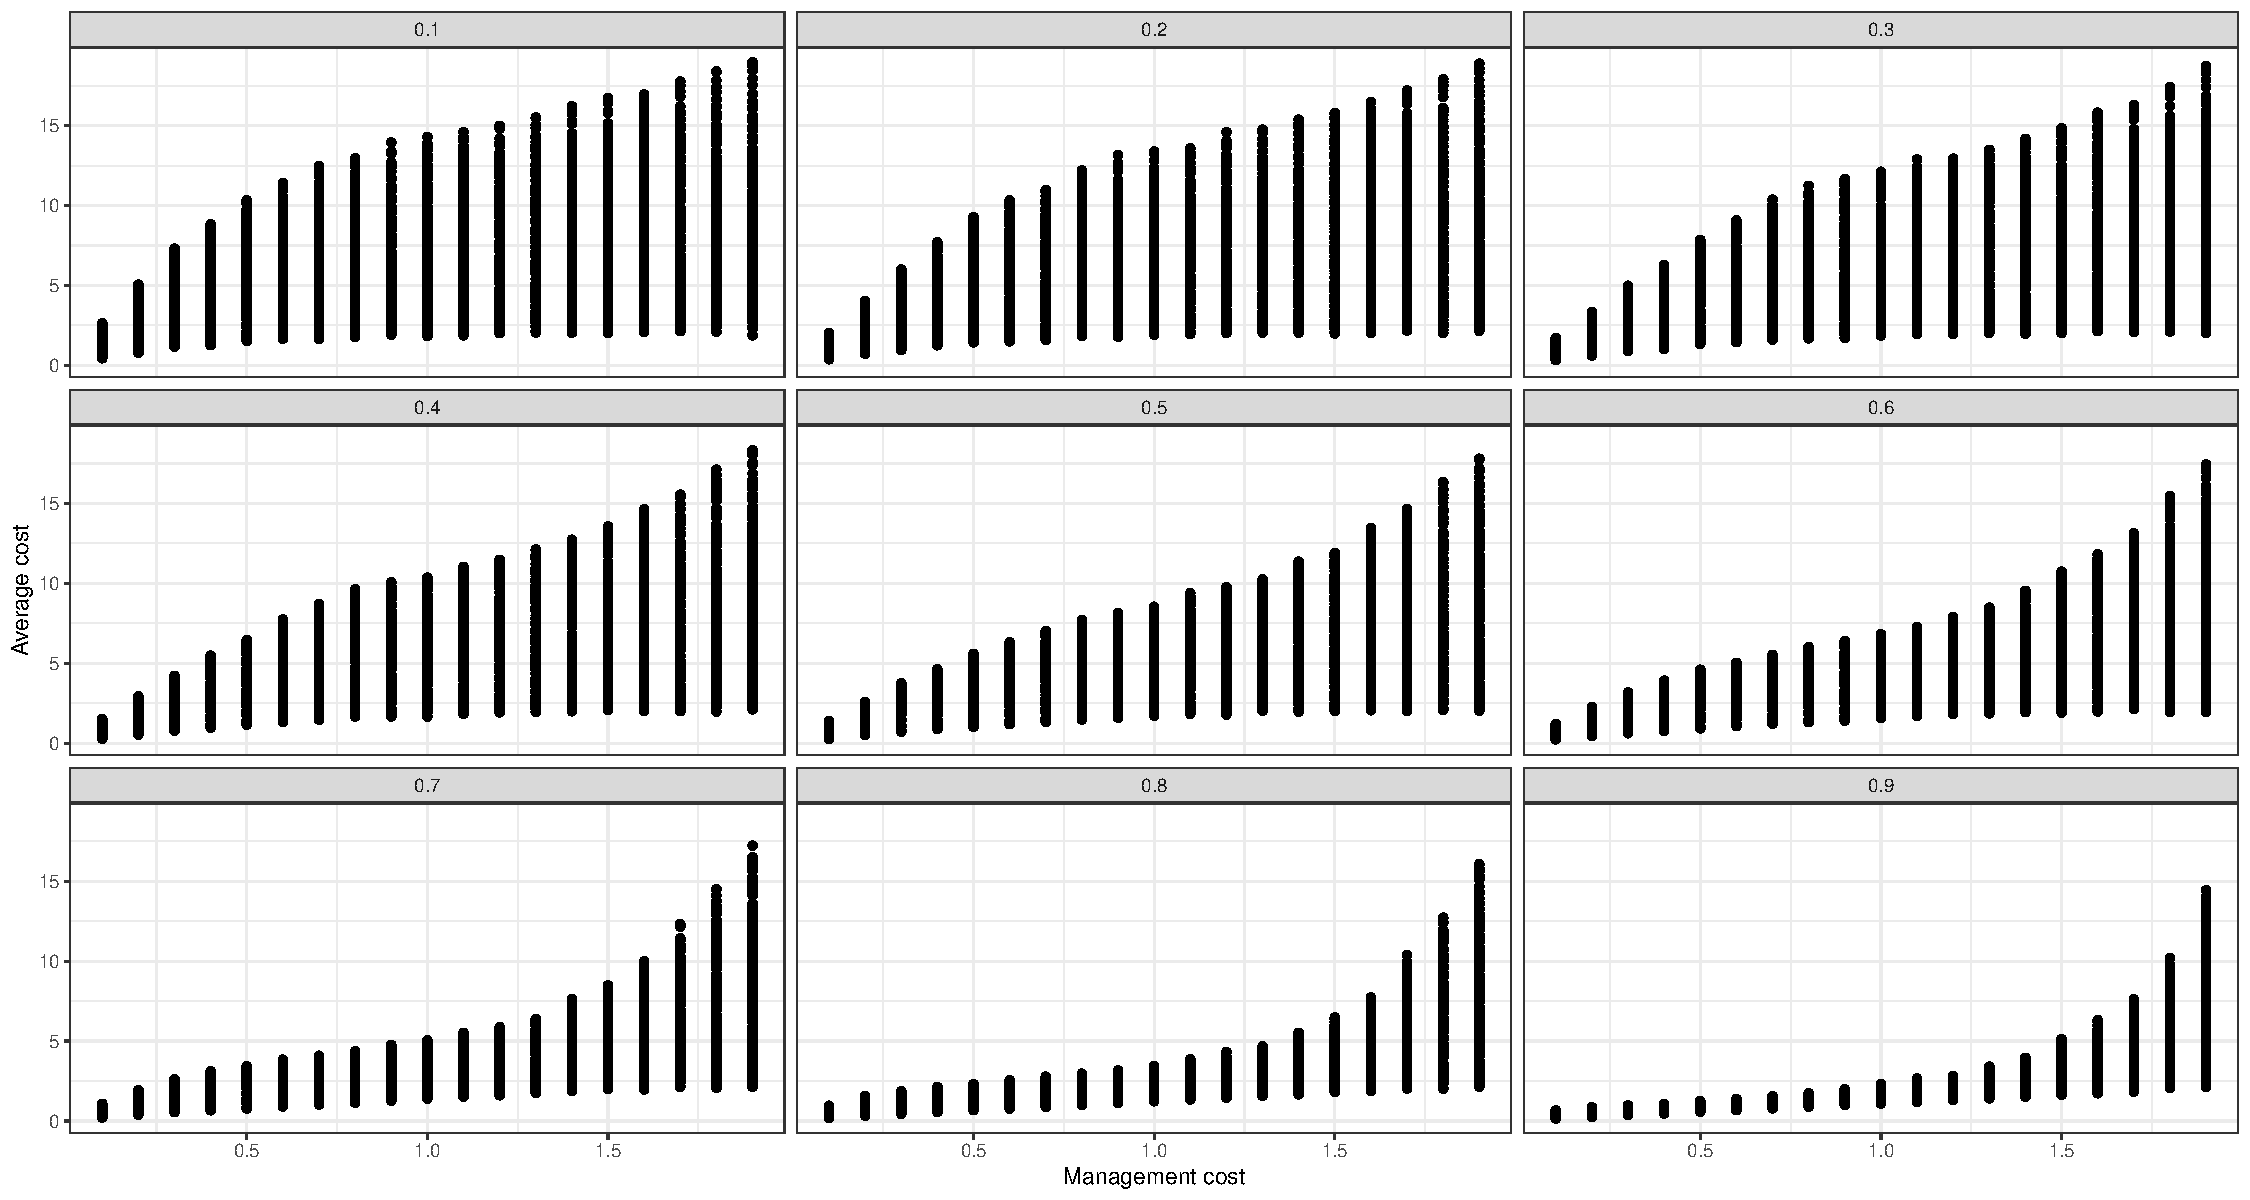
\includegraphics[width = \textwidth]{plots/avg_cost_by_management_cost.pdf}
\end{figure}


\begin{figure}
\caption{Average costs versus management costs, by model quality} \label{fig:fraction_of_tasks_done_by_human}
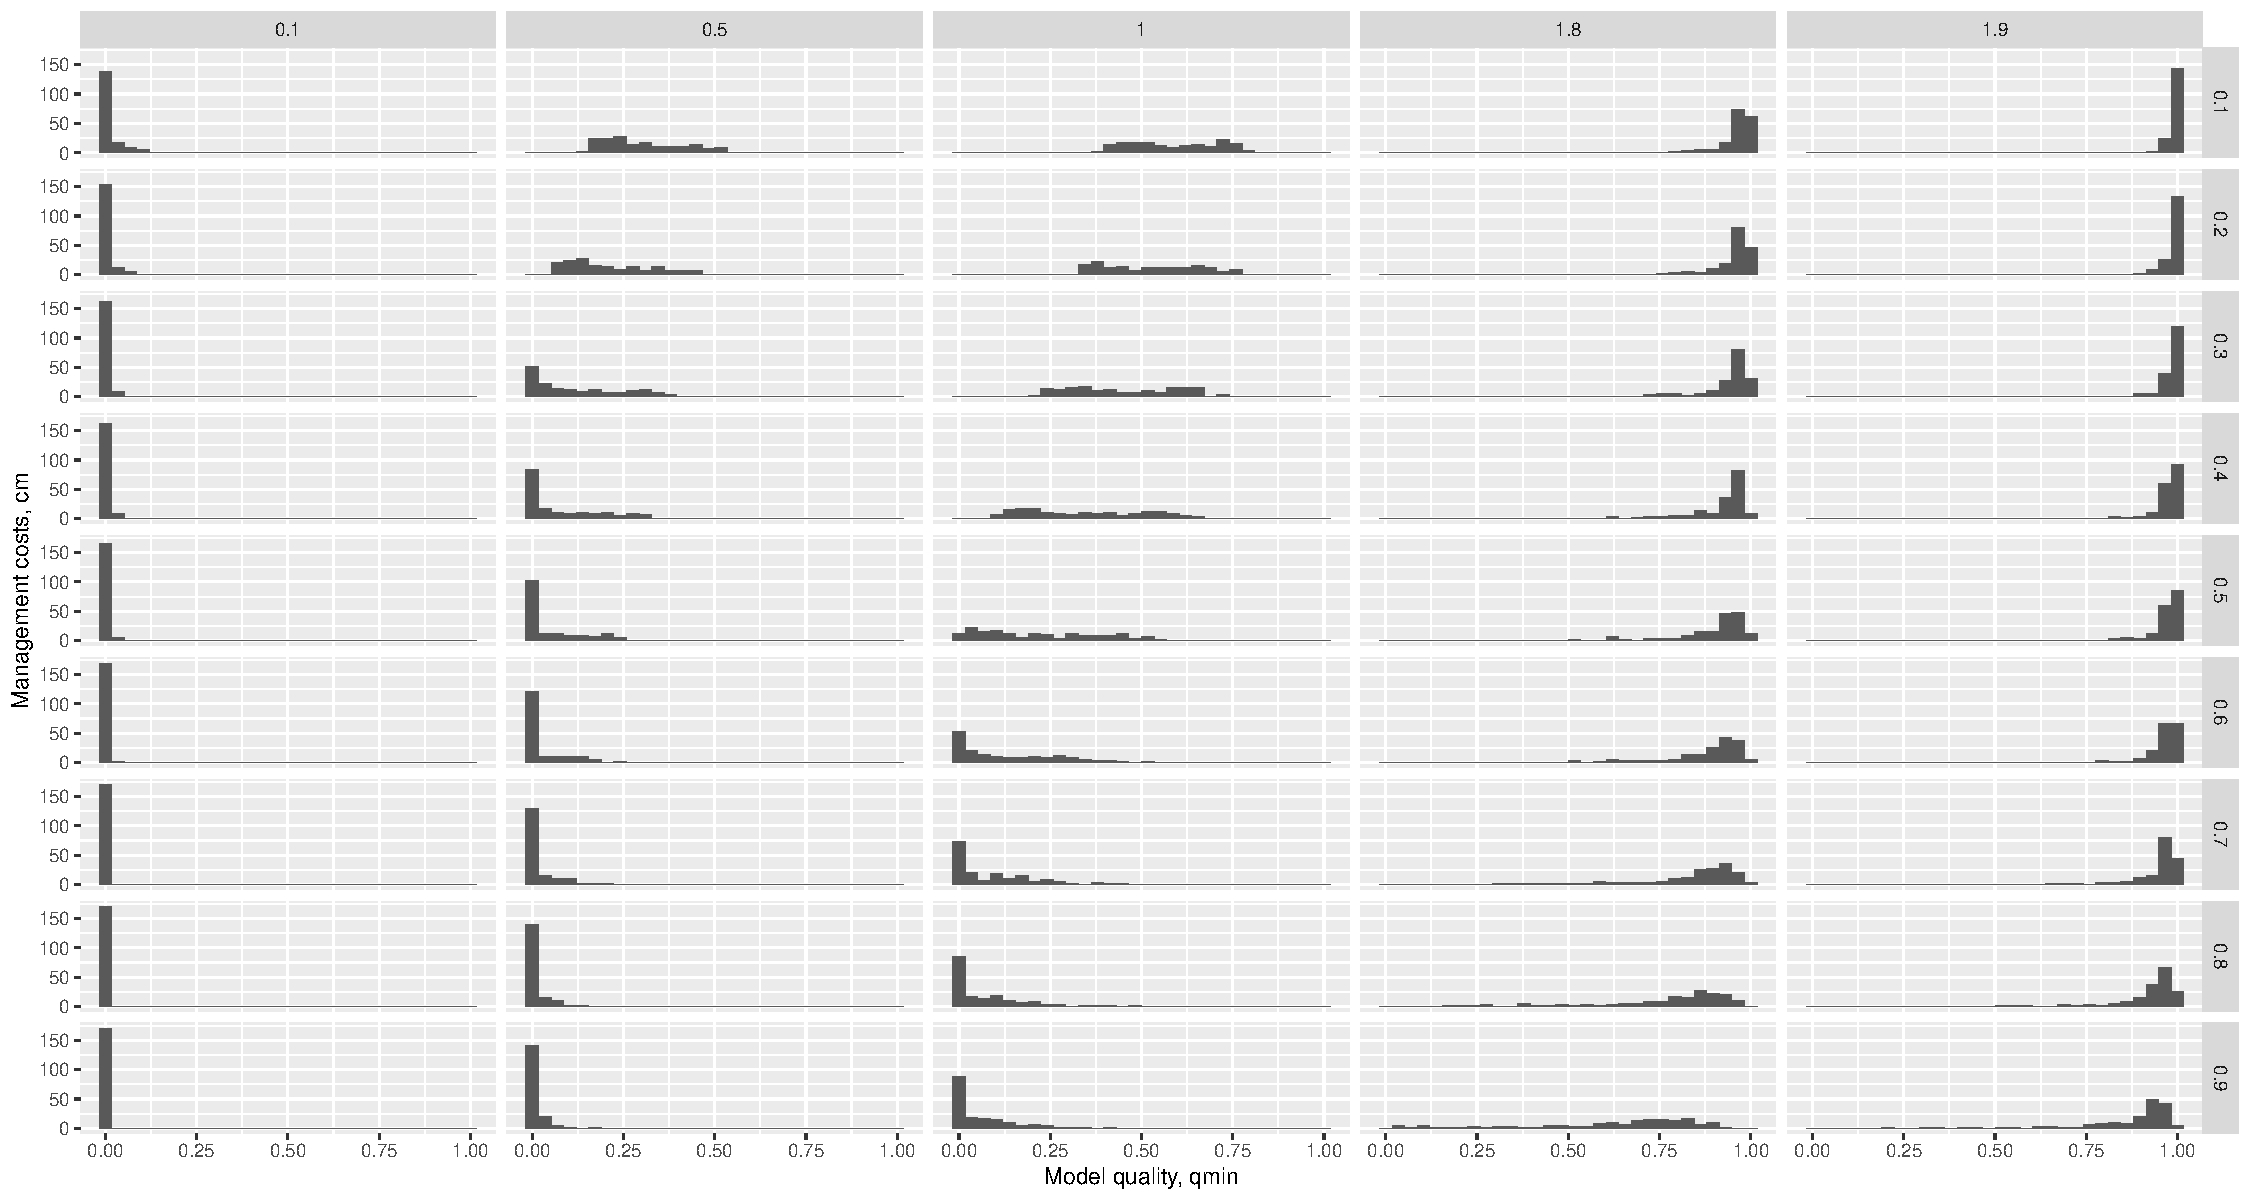
\includegraphics[width = \textwidth]{plots/fraction_of_tasks_done_by_human.pdf}
\end{figure}


\section{Discussion}

\subsection{So-so technologies}
Marginal tasks are those where $\cost{\machine{k}} \approx \cost{\human{k}}$.
If in constrast, $q = 0$ and goes to $1$, then $c_h - c_m$ could be quite large.
But the more exciting possibility is when we can chain.
Suppose we have $q_1 = 0$ and $q_3 = 0$ and $q_2 = 1$ and $q_4 = 1$.
We have $\human{1}\machine{2}\human{3}\machine{4}$, as a cost of $2c_h + 2c_m$.
If can improve $q_1$ and $q_3$ to 1, we can do $\machine{1}\machine{2}\machine{3}\machine{4}$,  we can get cost savings of $2 (c_h - c_m)$, leaving us with costs of $c_m$.
But if we consider the chaining possibility, letting us go to $\machine{1|2|3|4} $, we can go from $2c_h + 2c_m$ to just $c_m$. 

\subsection{What does ``full automation'' mean?}
Full automation consists of finding places in the production process where the costs of replacing the asking and evaluation steps with an AI are economical because the quality is sufficiently good and the cost of an evaluation failure is relatively low. 
For example, consider the task ``respond to customer inquiry'' previously done with a human representative. 
That human might take an inquiry and respond, perhaps with templates matching certain common questions and links to so-called knowledge-base articles. 
But even with a fairly rudimentary chatbot limited to a response of the form ``given your question, here are some resources you might find useful'' to replace this aspect of the customer service task.
The ``ask the AI to do something'' has been offloaded to the customer, as has the evaluation step is left to the consumer.
This full automation is just externalizing the prompting and evaluation costs to consumers, which presumably has some negative effect on demand.  

If the AI is doing the prompting and evaluation, we can think of $c_e$ and $c_p$ as de facto zero.
The failure mode is then the one step in the chain passes a bad prompt to the next. 
If the prompt and evaluation step has a very high $q$, this concern is not so great. 
Why do we not have an evaluation step? 
The prompt for the next task in the chain is the output from the previous step: there is no new effort, and this is already optimized to do that task as well as it can. 
There is also no distinct evaluation step. Why? 
Because if the AI could improve $q$ by evaluation on its own, that would already be included in the process it uses. 
The overall chain of unreliable components gives a $q = q_1 \cdot q_2 \cdot q_3$.
We can then consider just the human sandwich of prompting and evaluation, with this sequence of tasks in the middle.  

With a more advanced AI, it might try to answer a question directly.
This is common now. 
But it is unlikely that the task ``respond to current institutional investor inquiry'' would be turned over to even a sophisticated AI given the risks.

\subsection{AI usage as a managerial skill}
The routing, prompting, and evaluation tasks are similar to a manager's tasks.
Generative AI seems to complement a new kind of managerial skill, albeit the management of an AI. 
But given humans are harder to change the machines, it seems likely that AIs will continue to be modified to make it so that humans can manage them. 

Knowing what to yourself versus delegating, giving good instructions conditional upon delegating, and evaluating output---and course-correcting as necessary--- is closely similar to simply managing people.
Being a judge of talent, scoping and explaining projects in ways people will understand, giving good, actionable feedback, and so on. 
It is not fundamentally different from what should be delegated to a human. 

Adding ``let's think step by step'' to a prompt can dramatically increase performance \citep{kojima2023large}.

%% If instead of the AI producing the good costlessly, then some delegated worker has to do it. 
%% Suppose their wage is $w_1$, and they will take $t_1$ units of time.
%% A ``boundary of the job'' definition where a worker does the tasks is those where the costs of delegating to a specialist are greater than the cost savings. 
%% The difference is that when delegating to a worker, the costs are non-zero.
%% I do a task myself when $w_{0} t_{0} < (c_p + c_e + w_{1} t_{1})/q$.
%% I might delegate a task when (a) the person is higher-paid but must be more efficient (low $t_{1}$), the costs of managing are low (low $c_p$ and $c_e$), or the person is not as efficient by lower wage, $w_{1} < w_{1}$.

\subsection{Returns to more capable models}
Investments that raise task success probability, $q$, have two effects. 
They lower costs inframarginal for all tasks that the AI was already used for, with the elasticity of total costs equal to negative 1 in $q$, i.e., a 10\% increase in $q$ lowers expected AI costs by 10\%. 
The other effect is on the extensive margin, making some tasks more likely to be AI-able. 
The effect depends on the ``density'' of tasks where $q \approx \frac{c_p + c_e}{c_h}$, which presumably depends on the job.

\subsection{Returns to complementing the complementary skills}
The new tasks of routing, prompting, and judging are human tasks potentially complemented by AI. 
One interesting feature of LLMs is that with other investments, there are ``hacks'' that can lead to better performance. For example, asking the model to think ``step by step'' appears highly effective. 
And models that become knowledgeable about their own performance might be able to help design better prompts. 
For example, instead of a prompt ``What are good marketing slogans for an ice cream store?'' the prompt can be  ``what is a good prompt to an LLM that would generate good marketing slogans for an ice cream store?.''

Practices could also help with evaluation. 
For example, a request for a marketing slogan could also generate a collection of AI agents that will be asked to pretend to be customers.
They could then report their preferences. 
This would change the evaluation task to be more empirical. 

The other way that technological innovation can increase productivity is not by increasing model performance directly---working on $q$---but by lowering $c_p$ and $c_e$. 
These are innovations to make it easier to express what you want from machines and easier to evaluate outcomes seem likely. 

One interesting feature of the rise of ChatGPT is not that GPT3.5 was so much more capable than GPT3---it was that it had a user interface innovation that allows regular people to interact with an AI in a way that is similar to how they interact with people.
In a nutshell, OpenAI lowered $c_p$.

Becoming better at prompting will require the user to understand how to change the input to affect the model's output in the desired direction. 
We might think of the user as not so much choosing $x$ but as choosing an $x$ vector, with a greater understanding of the mapping between choices of $x$ and the outcomes.

\subsection{Evaluation costs}
Economics classifies goods by the actions consumers must take to assess them. 
Although it is a matter of degree, we can put goods roughly in order of the cost of evaluation

A company might be willing to try some LLM-generated ad copy in sponsored search ads with little to no human oversight; 
We might put more effort into evaluating a model's plan surgery or the draft of a judicial opinion.

\paragraph{Search goods}
For some tasks, the human is the final arbiter and can immediately decide if the outcome is sufficient.
There is no further source that needs to be considered.
For example, if a model is asked to ``come up with an agenda for a meeting to discuss recent sales declines'' the human can simply look at the agenda and decide if it is sufficient. 

\paragraph{Inspection goods}
There are other information goods that require a more costly inspection. 
As a case in point, consider computer code, which LLMs are good are producing. 
The user can then run that code to see if it runs correctly, with the caveat that it would be difficult to consider all possible inputs. 
This limitation aside, a popular paradigm in computer programming is ``test-driven development,'' where you create the tests first and then write the code, assessing automatically where it means your needs.

In solving certain kinds of math problems, the solution method is guess-and-verify. 
Or even if there is a routine procedure you follow, such as long division or solving an algebraic equation, we often switch mental modes to see if an answer is sensible. 
As an aside, many of the facile criticisms of Chat GPT take this form---show it is bad at giving you facts.  
AIs that can cite sources change inspection goods to search goods. 

The AI might lie to you, and, what you probably need to do is go verify the answer using normal research methods.

\paragraph{Information experience and credence goods}
Some information goods are consumed over time, and learning about the quality might take time. 
A person might not know if they enjoyed a movie until they have actually watched it. 
For information experience goods, we tend to rely heavily on reviews. 
But this only works when many people potentially evaluate the same good. 
With generative AI, the information good is likely generated uniquely for that particular worker. 
As non-lawyer could not verify whether a commercial contract is likely to hold up to scrutiny by the courts. 
A course of advised medical treatment might be very difficult to judge by a non-expert.


\paragraph{Rick Rubin Substitution: AI-enabled labor-labor substitution}

A low $c_h$ might imply a relatively $c_p + c_e$.

Knowing how to do something does not mean we have an advantage in asking people to do that thing, though we probably have an advantage in $c_e$.
But low $c_p + c_e$ does not imply a low $c_h$.

In the framing of the AI problem, we have assumed that the human who previously did the task was the one deciding whether to delegate that task to an AI. 
This could be sensible, but this is not necessary, and in fact, there could be advantages to using a different human for this task.
Consider that in the analogy to management, a person might delegate a task is precisely because they cannot do that task themselves. 

For judgment, as a heuristic, ``can do a task'' implies ``knowing if a task was done.''
This likely holds because a human performing some task is guiding that process to some outcome, and they presumably have to know where they are ``going.''
Even the simplest manual tasks have this property.  
A barista handing a customer a cup of coffee could release the cup in thousands of unique positions and times in 4D space-time, but only a very small subset of those leave the customer holding the cup and not scalded with spilled coffee. 
But $p \Rightarrow q$ does not imply $\neg p \Rightarrow \neg q$.
A person who had broken both arms could not hand a customer a cup of coffee but would still be able to know if a task was done.

There are likely to be numerous tasks when prompting and judgment can lead to good outcomes even when the human offering those judgments cannot do it themselves.
One reason is that the pool of people who can offer judgment is larger than the pool that can do the task. 
This might be particularly true for tasks that require a great deal of skill.
As a recent illustrative example,  the famed record product Rick Rubin described his value in a recent interview with Anderson Cooper:

\section{Conclusion}

\subsection{Why the details matter}
The history of technological innovation offers few completely general labor market lessons.
If there are any, they are the following: much of it tends to be labor-saving; jobs disappear, but work does not; complementary skills become more valuable, including whatever tasks humans still do \citep{autor2015there}. 
But it is difficult to know which particular jobs are impacted, what kinds of workers are complemented and what kinds are substituted, where productivity growth happens, and so on. 
For that, precisely what that technology does matters. 
For example, we have only made progress by getting into the details of say, what computers actually do and then exploring how this affects the productive process, as in \citep{autor2003skill}. 



\bibliographystyle{aer}
\bibliography{rubin}

\end{document}

``Explain the paradox of diamonds and water:''
\begin{quote}in that way, and I’ll start to understand.”
“But how do you explain how diamonds could be the only substance known to contain carbon? That’s a mystery.”
“Well, that’s easy. You go ahead and do it. I’ll tell you what I know. A diamond is the kind of thing that is made of carbon. It’s carbon-based. And like most things turned into diamonds, it’s a product of the same process that turns carbon into carbon.”
What is different is that they 
(it just goes on like this)
\end{quote}
And compare to GPT4
\begin{quote}
The paradox of diamonds and water, also known as the diamond-water paradox, is a classic illustration of the difference between total utility and marginal utility in economics. It was first introduced by classical economists in the 18th century.
The paradox is this: why is water, which is essential for life, so much cheaper than diamonds, which, while beautiful and rare, are not essential for survival?
The answer lies in the concepts of total utility and marginal utility.
(nails it)
\end{quote}


\end{document}

Polyani's paradox put limitations on what could be easily routinized.
The problem is that ``we know more than we can say''
Machine learning could help if it could see enough examples; we could teach it how to do certain things, even if we could not describe how we do them ourselves.
No one could write a program in the traditional way to ``identify a cat in a picture,'' but this turns out to be a relatively simple task with enough examples and the right kind of model--namely a neural network. 

If we could describe our judgment, it could be automated or included in the AI to increase $q$.


\subsection{Two labor market productivity effects from AI innovation}
Imagine a matrix mapping tasks to occupations, with the entries being the fraction of time spent on that task, in that occupation.
I.e., $d_{kj}$ would be the fraction of time spent on task $k$ in job $j$.

When a new AI capability emerges such that $t_y < t_v / q$ for some task $k$, this row is scaled down by $t_v/t_y$ for that task. 
The size of this effect depends how big $t_y$ is in various occupations, the number of such occupations, and the wage. 
This is the direct productivity effect of innovation on $k$. 
All the occupations that used $k$ have now grown more productive by the amount of time $k$ would take pre-AI innovation.

But there is also an indirect productivity effect that comes from a re-allocation of workers who previously had too-high of a $t_y$ for the task but have a sufficiently low $t_v$ that they can now do the task. 

If a task is becomes an AI task, some number of jobs might now have the same non-AI tasks.
In this case, labor supply can be used to fill the demand. 
Wages will equalized across the occupations, which means that workers will flow disproportionately into the occupation with the more elastic product market demand. 

\subsection{Model of jobs}
This is also a model of jobs. 
If the tasks do not need to be done in order---or there is a big enough lag---then you can send that task to someone else, who presumably can do it more efficiently. 
So the coordination cost has to be greater than the time time-savings. 
If I bake a cake, \begin{enumerate}
    \item I measure out the ingredients 
    \item mix them together
    \item Pour batter into the pan
\end{enumerate}
We could think of batter as an output of a productive process of ``measured out ingredients'' and ``mixing labor.''
The ``unbaked pan of batter'' as the output of the productive process ``batter'' and ``pouring labor.''
\begin{itemize}
\item $k_1 = \mbox{raw ingredients in bulk}$ 
\item $k_2 = \mbox{combined ingredients in right proportions}$
\item $k_3 = \mbox{batter}$
\item $k_4 = \mbox{pan with batter}$
\item $y = \mbox{cake}$
\item $l_1 = \mbox{measuring and combining}$
\item $l_2 = \mbox{mixing}$
\item $l_3 = \mbox{pouring}$
\item $l_4 = \mbox{shoving in oven}$
\end{itemize}
The productive process is 
\begin{align}
    y = f_4(k_4 = f_3(k_3 = f_2(k_2 = f_1(k_1, l_1), l_2), l_3), l_4)
\end{align}
I could, for example, split these jobs across multiple workers, with different workers providing each of the labor inputs. 
E.g., one station is doing the measuring, another doing the mixing, another is working the oven, and so on. 
I could also, at certain points, buy an intermediate good on the market rather than buying it myself. 
For example, I could buy cake mix and skip the measuring and mixing steps in the process. 

If we think a process is economically optimized, there should be no further gains from task division or buying on the market. 
I.e., if the market price of $k_3$, batter, is $p_3$ then $p_3 k_3$ is more than my ``make'' cost of $c_3 k_3$. 
I presumably have some cost advantage related to transaction costs. 
For example, for cake batter, if I bought it, I would have the pay the transportation costs. 
For something like cake batter that has a lot of water in it, this is expensive, whereas the bakery can transport water far more cheaply (namely by turning on a tap). 
Also, with batter purchased, I might have to have a freezer or refrigeration in a way that adds to costs, whereas batter I make myself, I can make it as needed. 

For labor, consider the $l_3$ ``pouring'' task. 
This might actually be both ``pouring'' and ``scraping the bowl.''
Now, one could imagine we split this into two steps so we can reap the benefits of specialization. 
This could simply reflect the cost of changing tools. 
For example, the scraper would need one of those rubber spatulae 

But there is some hand-off cost to doing this---imagine a Pouring Specialist waiting for a Scraping Specialist to come to get the last bit out of the bowl. 
Furthermore, the differences in productivity are not likely to be so great that this decomposition makes sense. 

So this task does not get further subdivided. 
This labor is actually both pouring 
I could also 




Let us suppose that the $c_h$ we discuss was actually just a measure of time. 
Let us suppose workers are paid their marginal product, and these completed tasks are worth $p$ in the product market.
Wages are about jobs, not tasks, but let's ignore that for now.
Hourly wages pre-AI are 
\begin{equation*}
    w_{PRE}= \frac{p}{\Bar{t}},
\end{equation*}
and with AI, suppose it is rational for the worker to use AI for $f$ of the tasks. 
The time it takes to do the same amount of work is now 
\begin{equation*}
    \Bar{t}_{post} = (1-f) \Bar{t} + f t_V /q
\end{equation*}
% tpost = (1-f)t + f tv/q  


\subsection{Setup}
Imagine a job as a sequence of tasks that must be done in order.
Let us suppose it takes $t_y$ to do a particular task yourself. 
An AI can try to do the task in no time at all. 
Ignore the cost of sending the task to the AI. But you do have to ``verify'' the output of the AI to decide if it is acceptable. 
This verification step is what we mean by judgment. 

This verification for that task takes $t_v$ units of time.
You might also think of verification as ``touching up'' the AI's work.
You know the probability the AI does it correctly for the task is $q$.
If the AI fails at the task (which happens with probability $1-q$), you can simply re-try, as failures are independent.
But with each try, you need to pay the verification cost again.
As such, the expected cost of using the AI is $t_v/q$.

\subsection{When you use AI for a task}
The condition for using an AI is a simple rule: is the first-shot success probability greater than my ratio of verification cost to performance costs, or:  
 \begin{equation}
     q> \frac{t_v}{t_y}.
 \end{equation} 

If an AI is still bad---a low $q$---you might try it if the expected cost savings are great.
The cost savings are great if verification is much less costly than production.    
\subsection{Examples: What tasks in a job are a low verification-to-production ratio?}
For a given job, for a given AI, what fraction of tasks has a low ratio, i.e., ``know it is right when you see it,'' but making it yourself is hard? 

Come up with an agenda for a meeting to discuss recent sales declines I can simply look at the agenda and decide if it meets my needs. 

Writing a letter to an employee that caused a workplace accident (something by dad used it for) Verification is simply reading the letter and seeing that it meets your needs. You are the arbiter of correctness.   

Does this code solve my problems (my main use case)
You just need the right boilerplate for a lot of programming to get something functioning. The machine helps you verify.


\subsection{Exploiting zero marginal costs with parallelism}
If the AI literally has zero performance costs, it might make sense for the model to create multiple versions of the output for the human to evaluate, particularly if $c_e$ is quite low and $q$ is quite low.

If $q$ really was a constant, the model should generate $\inf$ versions and let the user evaluate them serially, which would have expected costs $c_p + c_e/q$---one prompt and then as mean evaluations as needed until a success. 
The only reason the system would not do that is if we expect subsequent prompts following a failure to increase success probability. 

Suppose the first prompt has the probability of success $q_L$, and the second is $q_H = 1$, and because of this perfect second step, there is no evaluation cost.
The AI generates $k$ versions for the worker to evaluate---and the worker evaluates all of them.
The chance that all $k$ outputs are useless is $\approx \exp{-q_L k}$, in which case the second prompt is used $c_p$.
\begin{align}
  \min_k c_e k + c_p \exp{-q_L k}
\end{align}
Solving for the optimal $k$,
\begin{align}
    k^* = \frac{\log{\frac{c_p}{c_e}}  + \log q_L}{q_L}.
\end{align}

To exploit this parallelism strategy, prompting costs have to be larger than evaluation costs i.e., $c_p > c_e$.
Smaller evaluation costs push for larger $k$'s.
The effects of $q_L$ are ambiguous.
On the one hand, the lower the $q_L$, the greater the likelihood that no items are acceptable, and so increasing $k$ can prevent having to bear $c_p$. 
But each one is also worth less. 


\subsection{Is there a polynomial time algorithm for cost minimization?}
You have a collection of tasks, $T$, indexed by $i$.
At the start, assume each is done by a human i.e., $T_0 = \human{1}\human{2}\human{3}\ldots \human{n}$.
Let $C\{T\}$ be the cost of some allocation of machines and humans to a sequence of tasks, $T$.
\begin{enumerate}
\item For each task in $T$, decide if it should be done by a machine, even without any ``chaining.'' 
$C\{\machine{i}\} \le C\{\human{i}\}$.
Ignoring subscripts, this is just $c_{h} < c_{m} / q$.
\item Find $i$ with the largest value of $q_i + q_{i + 1}$ in $T_j$.
\item For that $i$, if $C\{\machine{i | i + 1}\}$ is the smaller than costs of of $\machine{i}\machine{i + 1}$, $\machine{i}\human{i+1}$, $\human{i}\machine{i + 1}$, ``chunk'' tasks $i$ and $i+1$. This means replace the $i$th position in $T$ with a new automated task with $q_{i'} = q_i q_{i+1}$. Delete the $i + 1$ position task.
\item Go back to step 2 and repeat. If $T_{j + 1} = T_{j}$, i.e., there are no more substitutions to produce, stop.
\end{enumerate}


\subsection{Direct productivity effects before equilibration}
Let us suppose that each task a worker does has a $(c_h, c_e, c_p, q)$.
The time worked was $C_H = \sum c_h$, for which the worker was paid $y$.
Their old wage was $w_{pre} = y / C_H$.
With an AI, they still do those where $c_h < (c_p + c_e)/q$; the rest are sent to the AI and done in $(c_p + c_e)/q$.
Let $f = Pr(c_h < (c_p + c_e)/q)$.
Let $C_{H/AI} = f \mathbf{E}[c_h | c_h < (c_p + c_e)/q]$ 
and 
$C_{AI} = (1 - f)\mathbf{E}[(c_p + c_e)/q | c_h > (c_p + c_e)/q]$.
The new wage before any equilibrium adjustment is thus 
\begin{align}
  \frac{w_{post}}{w_{pre}} = \frac{C_H}{  C_{H \setminus AI} + C_{AI} }
\end{align}

Before any equilibrium adjustment, wages increase as the average take to complete tasks can only go down.
The new average wage is higher.
Of course, what matters is the shape of the demand curve for the job that demands those tasks and what this does to p and entry on the supply side.
If demand for the tasks associated with a job is inelastic, you would get large reductions in wages, and vice versa if elastic.
